\chapter{Laboratorio 4}

Il primo circuito analizzato è il multivibratore monostabile (\Fig\ref{fig:circuito_1}). Tale circuito presenta uno stato stabile, in cui rimane fino a che un impulso esterno di comando lo porta in un secondo stato, in cui il circuito rimane per un tempo predefinito per poi tornare spontaneamente nello stato stabile, in attesa di un successivo impulso.
\begin{figure}[h]
	\centering
	\begin{minipage}{.45\textwidth}
		\scalebox{.62}{
			\begin{circuitikz}
				\draw (2,6) node[op amp, anchor=-](oa){\texttt{TL071}};
				\draw (oa.-) -- ++(-2, 0) coordinate (D) -- ++(-2,0) to[C=$C$] ++(0,-1.5) node[ground]{};
				\draw (D) to[D=$D$] ++(0,-1.5) node[ground]{};
				\draw (oa.up) -- ++(0, 0.3) node[vcc]{$V_{DD}$};
				\draw (oa.down) -- ++(0,-0.3) node[vee]{$V_{SS}$};
				\draw (oa.out) -- ++(1,0) coordinate(loop);
				\draw (loop) -- ++(0,-2.3) coordinate(R2) to[R=$R_2$] ++(-3.39,0) coordinate(rg) (R2-|oa.+) -- (oa.+);
				\draw (oa.-) -- ++(0,1.7) to[R=$R_3$]++(3.39,0) coordinate(Rf) (Rf-|loop) -- (loop);
				\draw (oa.+) to[short, -o] ++(0,0) ++(-.1,0) node[left]{$v_+$};
				\draw (oa.-) to[short, -o] ++(0,0) ++(0,-.1) node[below]{$v_-$};
				\draw (rg) -- ++(-1,0) coordinate(r1) to[R=$R_1$] ++(0,-2) node[ground]{};
				\draw (r1) to[D=$D_T$] ++(-2.5,0) coordinate(vt) to[C=$C_T$] ++(-3,0) coordinate(vin);
				\draw (vt) to[R=$R_T$] ++(0,-2) node[ground]{};
				\draw (vt) to[short, -o] ++(0,0) node[above]{$v_t$};
				\draw (loop) to[short, -o] ++(0,0) ++(.1,0) node[right]{$v_{out}$};
				\draw (vin) to[sqV=$v_{in}$] ++(0,-2) node[ground]{};
				\draw[thick] (-5.5,0) rectangle (6.5,8.5);
			\end{circuitikz} 
		}
	\end{minipage}\qquad
	\begin{minipage}{.45\textwidth}
		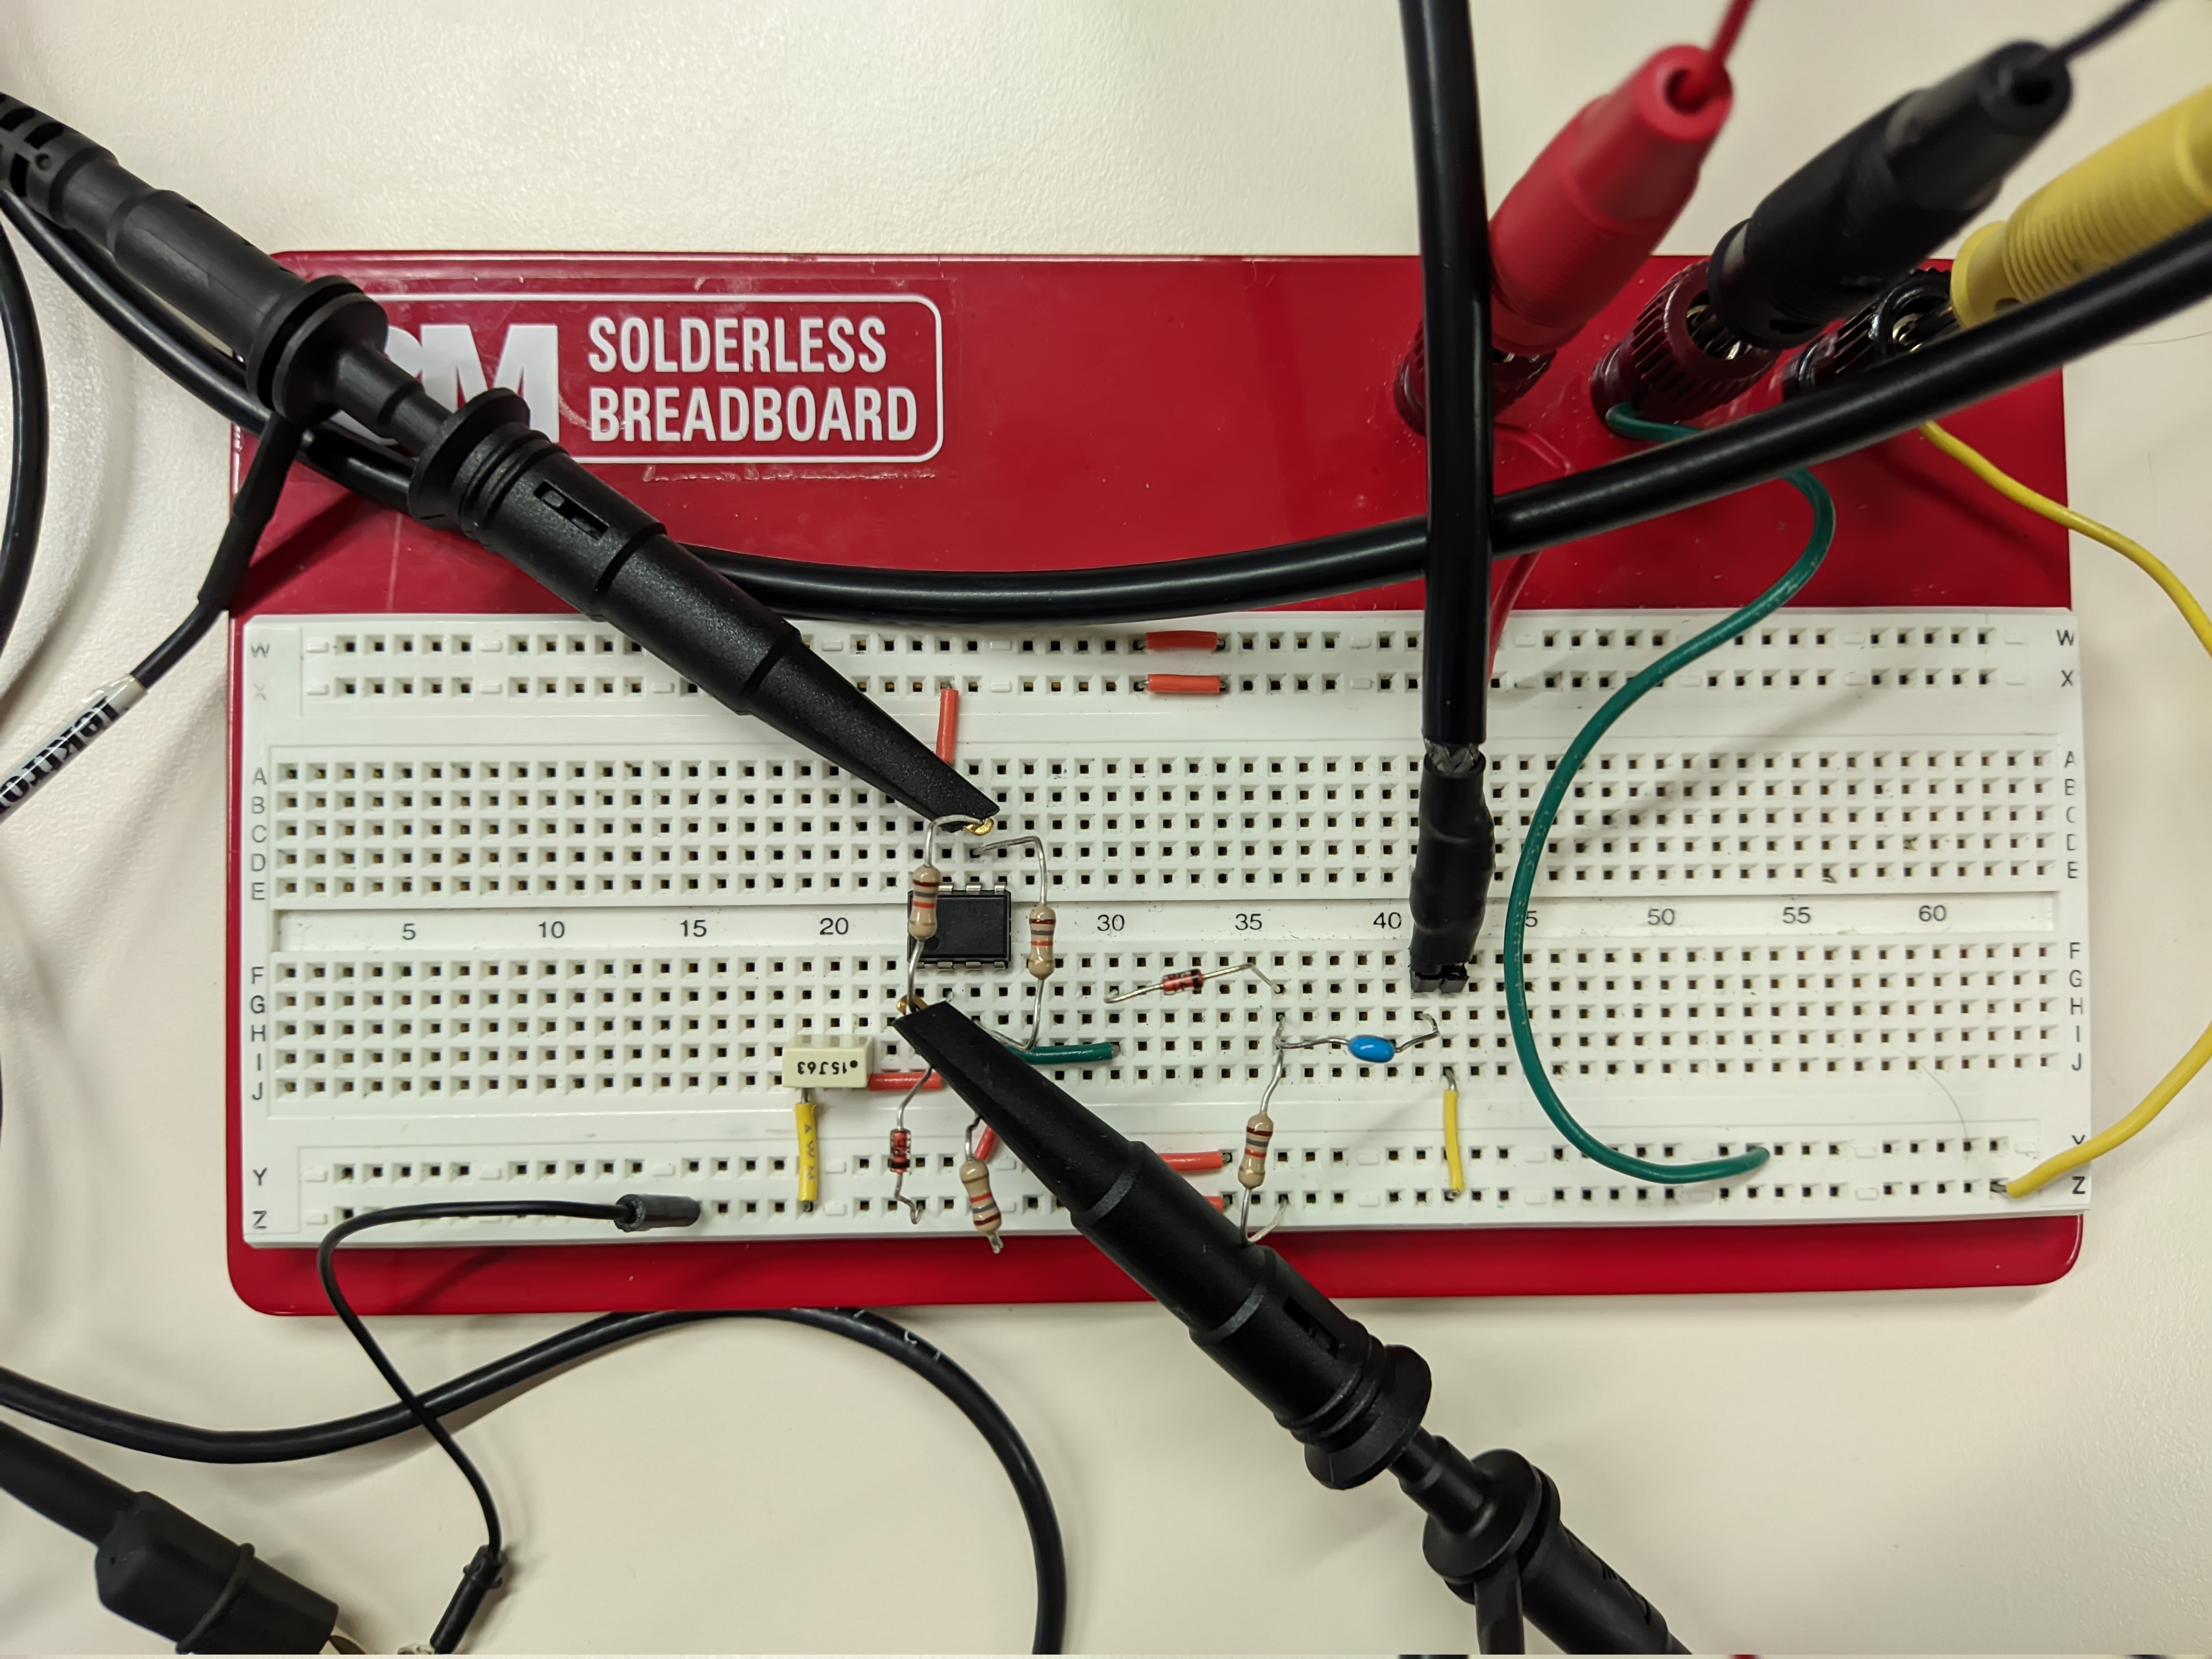
\includegraphics[width=\linewidth]{./ImageFiles/Laboratorio 4/CIR11.jpg}
	\end{minipage}
	\caption{Schema circuitale del multivibratore monostabile e foto del circuito realizzato.}
	\label{fig:circuito_1}
\end{figure}
Per realizzare il circuito, si parte dal generatore d'onda quadra visto nella precedente esperienza di laboratorio. Inserendo un diodo $D$ in parallelo alla capacità $C$ si ottiene uno stato stabile. Supponiamo che inizialmente la tensione di uscita sia pari a V\sub{DD} e che la capacità sia scarica. Allora, la capacità si carica attraverso la resistenza R\sub{3} fino a quando la tensione ai suoi capi raggiunge circa \SI{0.7}{\volt} (tensione di polarizzazione del diodo $D$). A questo punto, il processo di carica si interrompe perché il diodo si accende e si comporta come un cortocircuito. Quindi la corrente scorrerà solo attraverso il diodo $D$ verso massa. Quindi l'uscita rimane stabile alla tensione V\sub{DD}.

\noindent
Affinché il circuito commuti dallo stato stabile $v_{out}=V_{DD}$ allo stato quasi stabile $v_{out}=V_{SS}$ è necessario che la tensione dell'ingresso non invertente scenda al di sotto della tensione dell'ingresso invertente. Questo viene reso possibile applicando sul morsetto non invertente un impulso negativo di tensione. Per fare ciò si inserisce un circuito derivatore composto da una capacità $C_T$ ed una resistenza $R_T$. Tale circuito ha il compito di generare, a partire da un segnale rettangolare $v_{in}$, un impulso positivo ed uno negativo. Questi \textit{spike} di tensione sono generati sui fronti di salita e discesa dell'onda quadra in ingresso. Il diodo $D_T$ permette di non trasmettere gli impulsi positivi al nodo V\super{+} (il diodo infatti si spegne) ma lascia passare inalterati gli impulsi negativi.
Questo impulso negativo generato porterà per un breve istante la tensione $v_+$ al di sotto della tensione presente ai capi del condensatore (che è pari alla tensione di polarizzazione del diodo) forzando la commutazione dell'uscita a $v_{out}=V_{SS}$. A questo punto, il condensatore si scarica fino a raggiungere la tensione di soglia $V_H^+=\frac{1}{2}V_{SS}$ dove l'uscita commuta portandosi a $v_{out}=V_{DD}$. Il condensatore ricomincia così il ciclo di carica ma termina una volta raggiunta la tensione di polarizzazione del diodo (che è minore della nuova tensione di soglia V\sub{H}\super{+}) . Il circuito entra di nuovo in uno stato stabile in attesa che sul morsetto non invertente venga generato un altro impulso negativo. Il tempo per cui $v_{out}=V_{SS}$ dipende dalla capacità $C$ e dalla resistenza $R3$.

\noindent
I valori utilizzati nel circuito sono indicati nella tabella \ref{tab:valori_componenti_1}. L'amplificatore scelto è il \textbf{TL071} ed è stato alimentato con una tensione duale di $\pm$\SI{10}{\volt}.

\def\arraystretch{1.3}
\begin{table}[h!]
	\centering
	\begin{tabular}{|c|c|c|}
		\hline
		Componente	& Valore Nominale & Valore Misurato \\ \hline
		R1 &\SI{18}{\kilo\ohm} & \SI{17,96}{\kilo\ohm} \\ \hline
		R2 &\SI{18}{\kilo\ohm} & \SI{17,79}{\kilo\ohm} \\ \hline
		R3 & \SI{18}{\kilo\ohm} & \SI{18}{\kilo\ohm} \\ \hline
		R\sub{T} & \SI{18}{\kilo\ohm} & \SI{17,83}{\kilo\ohm} \\ \hline
		D\sub{T} & $\simeq$\SI{0.7}{\volt} & \SI{609}{\milli\volt} \\ \hline
		D1 & $\simeq$\SI{0.7}{\volt} & \SI{607}{\milli\volt} \\ \hline
		C & \SI{150}{\nano\farad} & Non misurato \\ \hline
	\end{tabular}
	\caption{Valori nominali e misurati dei componenti utilizzati nel circuito.}
	\label{tab:valori_componenti_1}
\end{table}

\noindent
Per generare gli impulsi di tensione, si è utilizzato un segnale in ingresso ad onda quadra con \textit{duty-cicle} pari al 20\%, frequenza di \SI{100}{\hertz} e ampiezza picco-picco pari a \SI{5}{\volt}\todo{Inserire valori corretti}. In figura \ref{fig:picchi_ingresso} si vedono i picchi generati dal derivatore. 

\begin{figure}[h!]
	\centering
	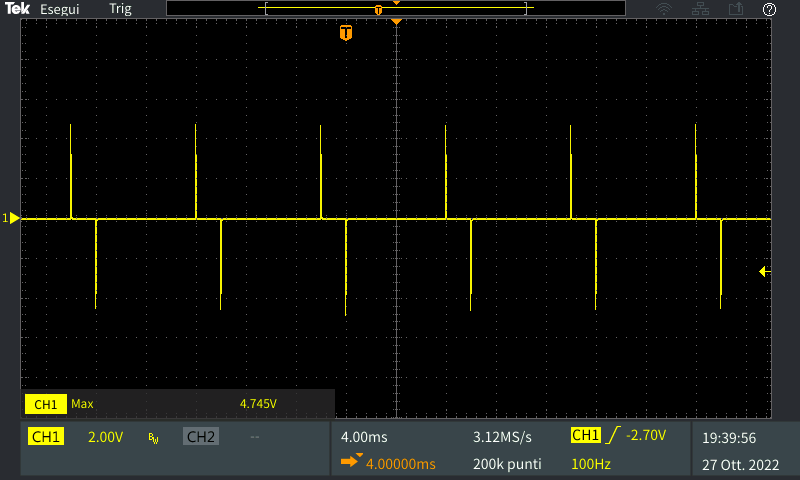
\includegraphics[width=\linewidth]{./ImageFiles/Laboratorio 4/TEK00002.PNG}
	\caption{Misure del segnale $v_{t}$ (linea gialla). Questi picchi sono generati dal circuito derivatore con in ingresso un'onda quadra con \textit{duty-cicle} del 20\%, frequenza di \SI{100}{\hertz} e ampiezza picco-picco pari a \SI{10}{\volt}.}
	\label{fig:picchi_ingresso}
\end{figure}

\noindent
In figura \ref{fig:segnale_uscita} sono invece mostrati gli andamenti di $v_{-}$ e $v_{out}$. È interessante notare che i valori di saturazione dell'amplificatore operazionale, e quindi i valori tra cui commuta $v_{out}$, sono minori delle tensioni di alimentazione $V_{DD}$ e $V_{SS}$.
\begin{figure}[h!]
	\centering
	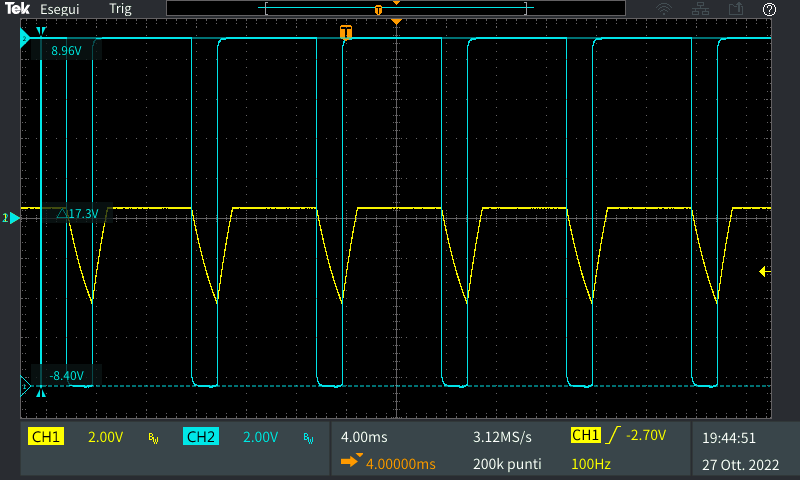
\includegraphics[width=\linewidth]{./ImageFiles/Laboratorio 4/TEK00008.PNG}
	\caption{Misure del segnale $v_{-}$ (linea gialla) e del segnale $v_{out}$ (linea azzurra).}
	\label{fig:segnale_uscita}
\end{figure}

\noindent
\`E stato inoltre possibile misurare il tempo in cui l'uscita rimane alla tensione V\sub{SS} (che indichiamo con T\sub{A}). Infatti, esso dipende dalla costate di tempo di carica e scarica $\tau=R_3C$ e dai valori delle resistenze R\sub{1} e R\sub{2}. Infatti, indicando con t\sub{1} l'istante in cui la tensione la nodo V\super{-} raggiunge la tensione soglia V\super{L}\super{+} e considerando t\sub{0} l'istante in cui viene applicato l'impulso negativo si ha che
\begin{equation}
	V^-(t_1)=V_{SS}+(\SI{0.7}{\volt}-V_{SS})e^{\frac{-t_1}{\tau}}=V_L^+
\end{equation}
e quindi, considerando $|V_{SS}|\gg\SI{0.7}{\volt}$ si ottiene
\begin{equation}
	t_A=\tau\ln\left(1+\frac{R_2}{R_1}\right).
	\label{eq:ta}
\end{equation}
Attraverso i cursori forniti dall'oscilloscopio si ricava che il tempo t\sub{A} è pari a \SI{1.78}{\milli\second} (\Fig\ref{fig:calcolo_ta}), mentre il valore teorico dato dall'equazione \ref{eq:ta} è di \SI{1.86}{\milli\second}.

\begin{figure}[h!]
	\centering
	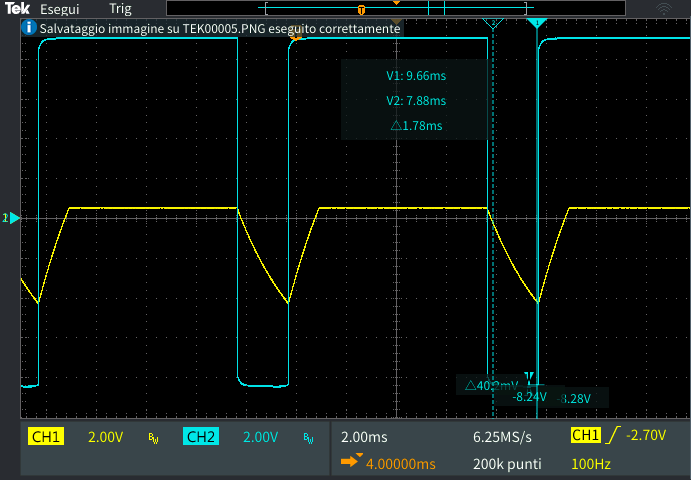
\includegraphics[width=\linewidth]{./ImageFiles/Laboratorio 4/TEK00006.PNG}
	\caption{Misure del segnale $v_{-}$ (linea gialla) e del segnale $v_{out}$ (linea azzurra).}
	\label{fig:calcolo_ta}
\end{figure}

\clearpage
Il secondo circuito visto a lezione è una variante del circuito precedente che implementa la funzione di un multivibratore monostabile tramite l'utilizzo dell'integrato \textbf{LM555} (\Fig\ref{fig:circuito_2}).
\begin{figure}[h!]
	\centering
	\begin{minipage}{.45\textwidth}
		\scalebox{.47}{
			\begin{circuitikz}
				%Main dip package
				\draw (0,0) node[dipchip,num pins=8, hide numbers, external pins width=0.1, scale=3, external pad fraction=6](C){LM555};
				%Pin names
				\node [right] at (C.bpin 1) {GND};
				\node [right] at (C.bpin 2) {TRIG};
				\node [right] at (C.bpin 3) {OUT};
				\node [right] at (C.bpin 4) {RST};
				\node [left] at (C.bpin 5) {CV};
				\node [left] at (C.bpin 6) {THRS};
				\node [left] at (C.bpin 7) {DISCH};
				\node [left] at (C.bpin 8) {$V_{CC}$};
				%Connections
				\draw (C.pin 1) -- ++(-4,0) -- ++(0,-6) node[ground]{};
				\draw (C.pin 8) -- ++(2,0) coordinate(vcc) -- ++(0,1.35) node[vcc]{$V_{CC}$};
				\draw (C.pin 7) -- ++(2,0) coordinate(dsc) to[R=$R$] (vcc);
				\draw (C.pin 6) -- ++(2,0) coordinate(trs) -- (dsc);
				\draw (trs) -- ++(2,0) to[C=$C$] ++(0,-2.68) node[ground]{};
				\draw (C.pin 5) -- ++(2,0) to[C=$C_2$] ++(0,-1) node[ground]{};
				\draw (C.pin 4) -- ++(-1.5,0) -- ++(0,3) to[crossing] ++(0,.72) to[crossing] ++ (0,2.64) node[vcc]{$V_{CC}$};
				\draw (C.pin 3) to[short, -o] ++(-1,0) ++(0,.1) node[above]{$v_{out}$};
				\draw (C.pin 2) -- ++(-3,0) coordinate(vin);
				\draw (vin) to[sqV=$v_{in}$] ++(0,-2) node[ground]{};
				\draw[thick] (-7.5,-5.3) rectangle (8,5.9);
			\end{circuitikz}
		}
\end{minipage}\qquad
\begin{minipage}{.45\textwidth}
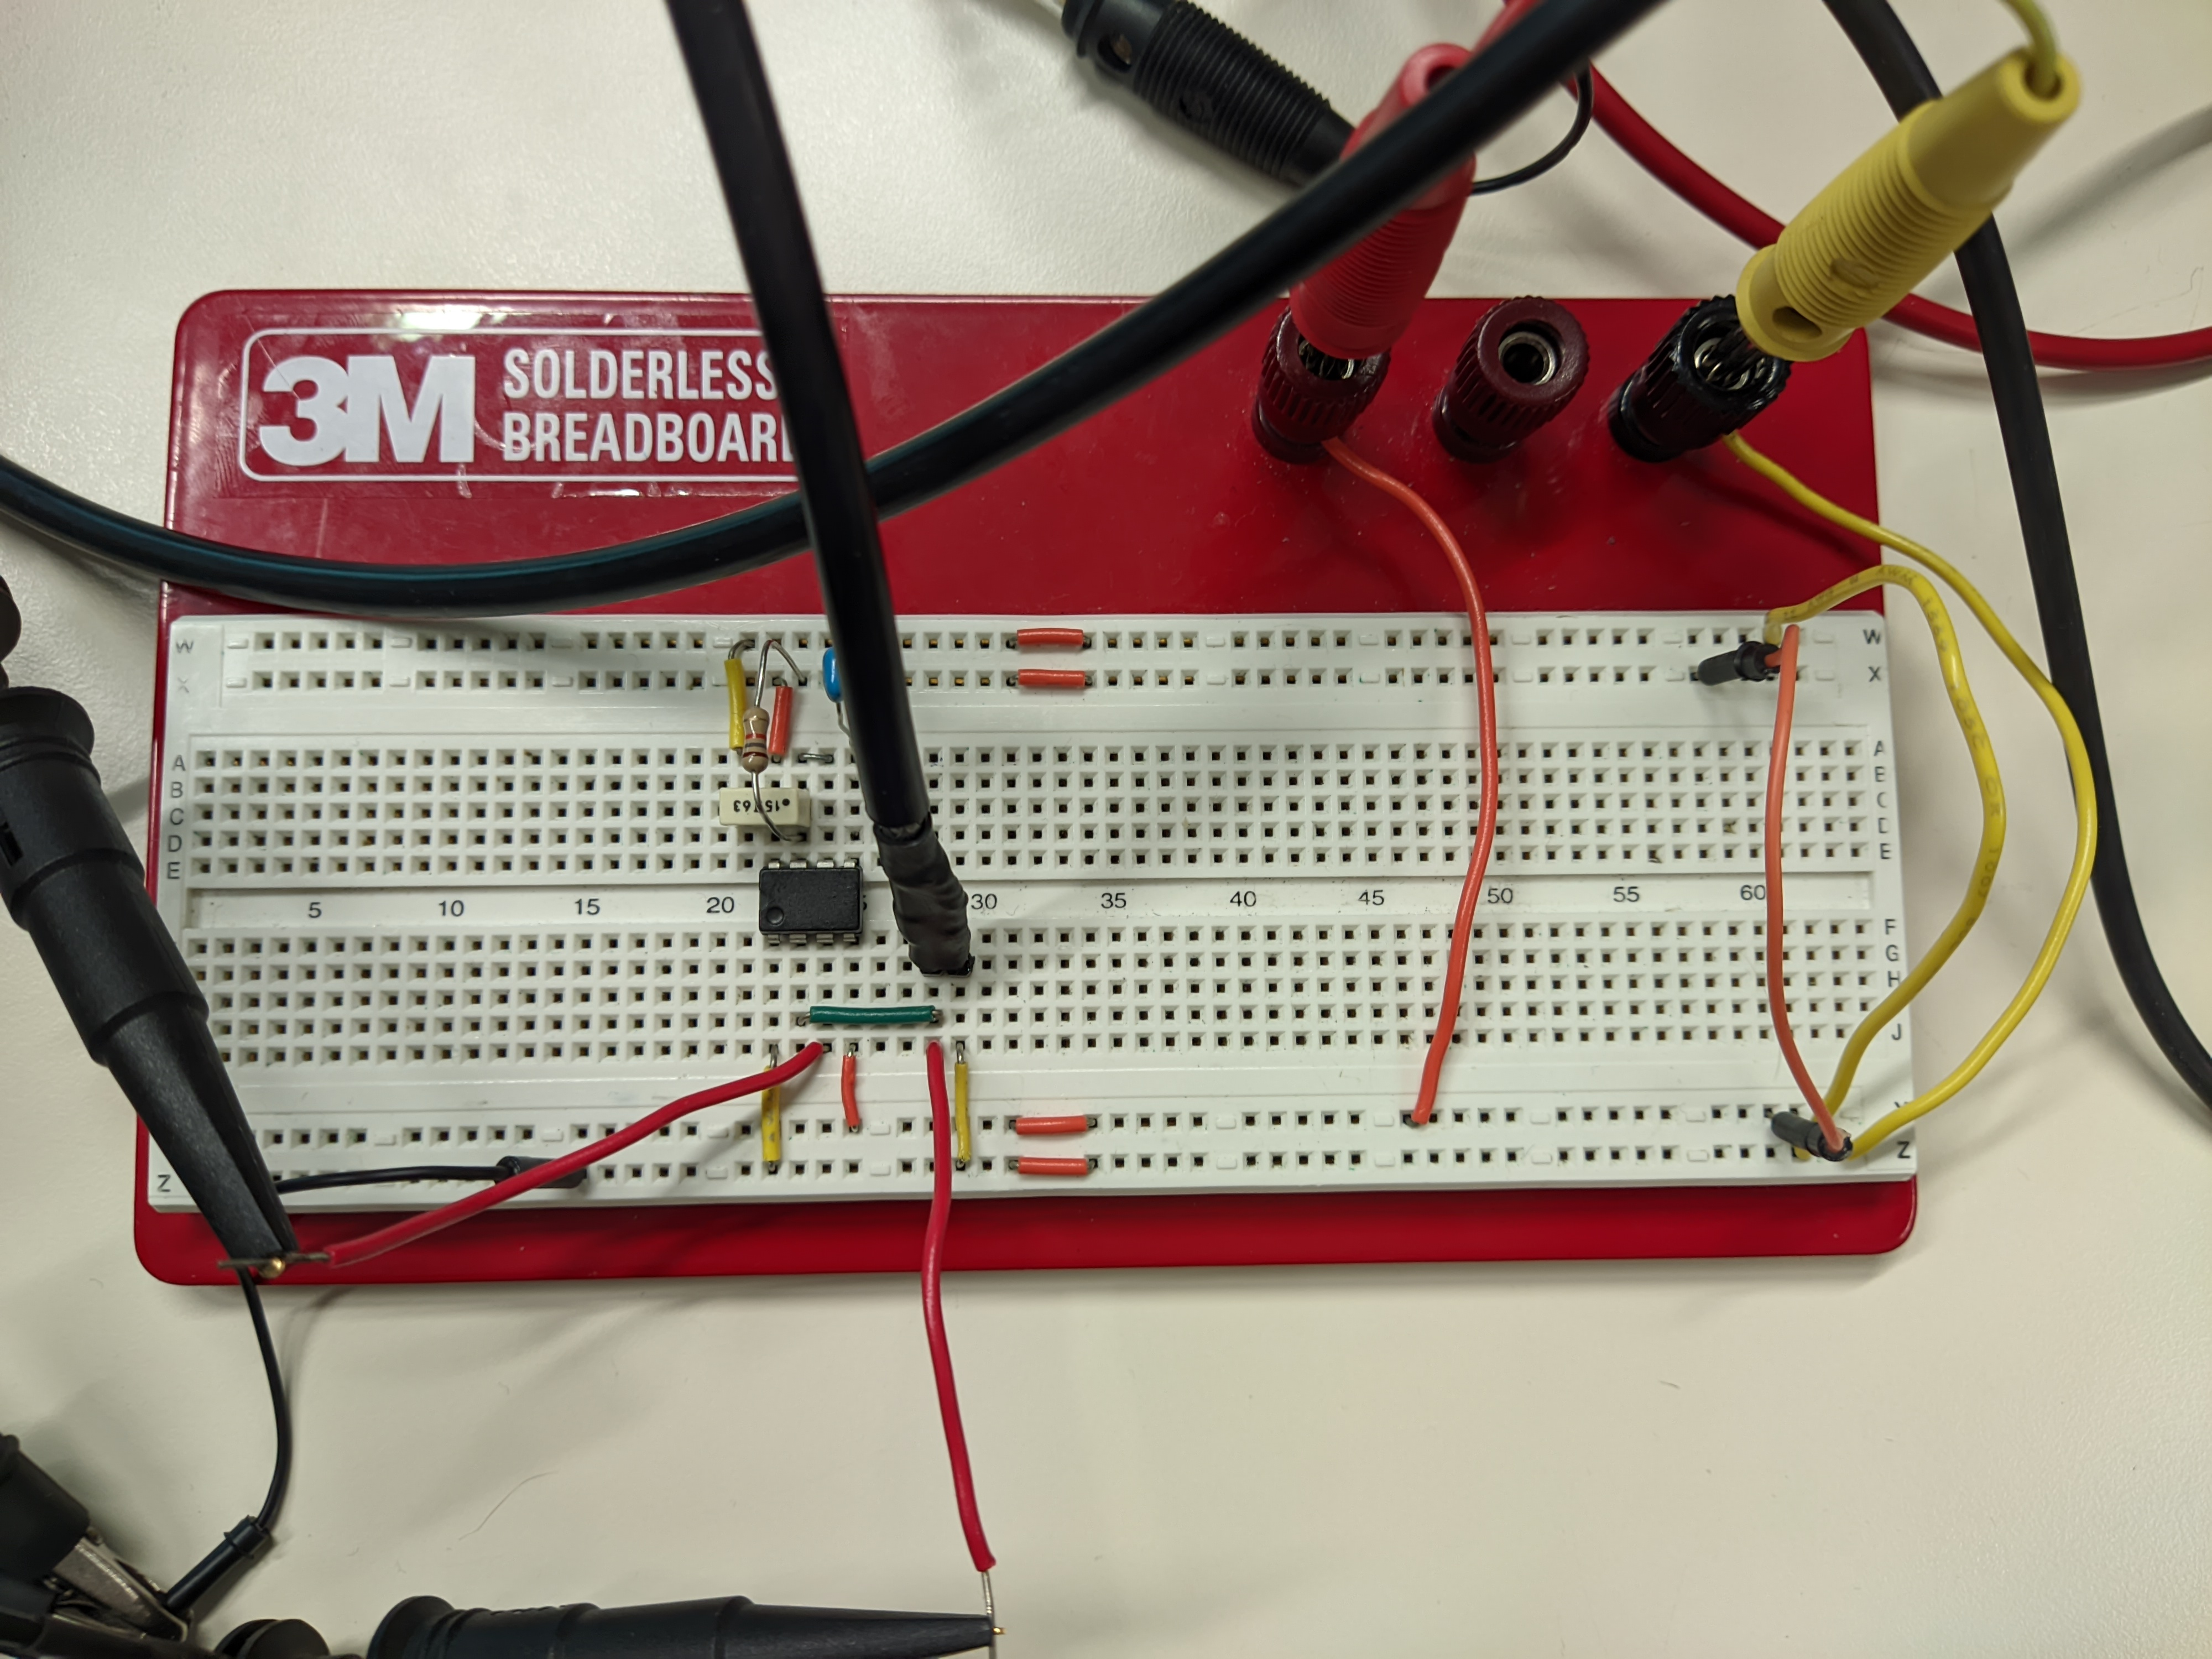
\includegraphics[width=\linewidth]{./ImageFiles/Laboratorio 4/CIR21.jpg}
\end{minipage}
\caption{Schema circuitale del 555 monostabile e foto del circuito realizzato.}
\label{fig:circuito_2}
\end{figure}

\noindent
Come si può osservare nella figura \ref{fig:555_internals}, \textbf{LM555} è composto da due comparatori, le cui uscite sono collegati ai morsetti di \textit{reset} e \textit{set} di un \textit{flip-flop}. Il pin \textbf{output} dell'integrato, è collegato tramite un porta NOT, all'uscita negata del \textit{flip-flop}. Inoltre, il pin \textit{Discharge} è collegato al collettore di un bipolare, in cui la base è anch'essa collegata all'uscita negata del \textit{flip-flop} e l'emettitore a massa. Ciò comporta, che quando \textbf{$\overline{Q}$} è a livello logico alto, il transistor si comporta come un corto, collegando a massa il pin \textit{Discharge}. 

\begin{figure}[h!]
	\centering
	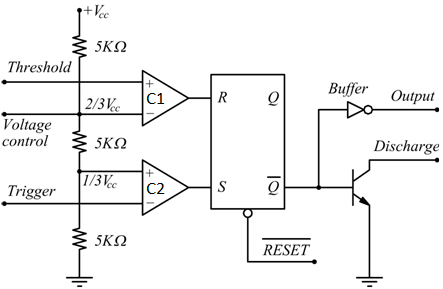
\includegraphics[width=0.6\linewidth]{./ImageFiles/Laboratorio 4/555internals.jpg}
	\caption{Struttura interna di un circuito integrato LM555.}
	\label{fig:555_internals}
\end{figure}

\noindent
Al comparatore \textbf{C1} è collegato il pin \textit{Threshold} all'ingresso non invertente mentre all'ingresso invertente è fornita una tensione costante pari a $\frac{2}{3}V_{CC}$, grazie al partitore formato tra tre resistenze in serie da \SI{5}{\kilo\ohm}. Il comparatore \textbf{C2} presenta una tensione costante pari a $\frac{1}{3}V_{CC}$ sul morsetto non invertente, mentre il morsetto invertente è collegato al pin di \textit{Trigger}.
Per capire il funzionamento del circuito realizzato è necessario ricordare la tabella di verità del \textit{flip-flop set-reset} \ref{tab:flip_flop_states}:

\def\arraystretch{1.3}
\begin{table}[h!]
	\centering
	\begin{tabular}{|c|c|c|}
		\hline
		S	& R & Q \\ \hline
		0 & 0 & Stato precedente  \\ \hline
		1 & 0 & 1\\ \hline
		0 & 1 & 0\\ \hline
		1 & 1 & Stato proibito \\ \hline
	\end{tabular}
	\caption{Tabella di verità di un \textit{flip-flop set-reset}.}
	\label{tab:flip_flop_states}
\end{table}

\newpage
\noindent
Analizziamo ora il comportamento del circuito. Supponiamo che inizialmente l'uscita \textit{v\sub{out}} sia a livello logico basso (\SI{0}{\volt}). Per cui, $\overline{Q}$ è a livello logico alto, accendendo il transistor di scarica. La differenza di tensione ai capi del condensatore C è quindi nulla e il condensatore è scarico. Inoltre, il segnale di trigger è mantenuto a una tensione pari a V\sub{CC}. Per cui, l'uscita del comparatore \textbf{C2} è a livello logico basso (S=0) così come quella del comparatore \textbf{C1} (R=0). Quando sul morsetto di trigger è applicato un impulso negativo (con picco minore della soglia $\frac{1}{3}V_{CC}$), l'uscita del comparatore \textbf{C2} cambia stato (S=1) in quando $V^+>V^-$. Per cui $\overline{Q}=0$ mentre l'uscita $v_{out}$ si porta a livello logico alto. Pe cui, il transistor di scarica si spegne e la capacità inizia a caricarsi tramite la resistenza R. Il processo di carica continua, fino a quando la tensione al nodo THRS supera la soglia $\frac{2}{3}V_{CC}$. A questo punto, il comparatore \textbf{C1} cambia stato (R=1) e porta quindi $\overline{Q}$ a livello logico alto e $v_{out}$ ritorna a 0. Per cui, il transistor di scarica si riaccende e porta la capacità a scaricarsi velocemente, riportando il nodo di \textit{Threshold} a 0. L'uscita quindi rimane stabile a livello logico basso fino a quando verrà applicato un altro segnale di trigger. Il funzionamento è riassunto in figura \ref{fig:555_mono}. Si noti che la capacità C\sub{2} è utilizzata per filtrare eventuali disturbi presenti sulla alimentazione.
\begin{figure}[h]
	\centering
	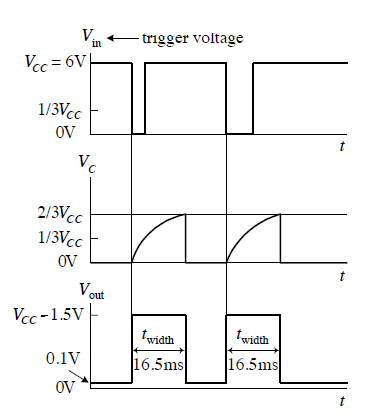
\includegraphics[width=0.5\linewidth]{./ImageFiles/Laboratorio 4/timer555}
	\caption{Funzionamento del LM555 in modalità monostabile.}
	\label{fig:555_mono}
\end{figure}

\noindent
Il tempo T\sub{1} di carica del condensatore varia in base ai valori di $R$ e di $C$, seguendo la relazione
\[v_C(t) = V_{CC}\cdot\left(1-e^{-\frac{t}{RC}}\right)\]

La carica della capacità termina quando $v_C = \frac{2}{3}V_{CC}$, quindi
\begin{equation}
	\begin{split}
		\frac{2}{3}V_{CC} &= V_{CC}\cdot\left(1-e^{-\frac{T_1}{RC}}\right) \\
		T_1&=-RC\ln\left(\frac{1}{3}\right)\approx1.1RC \\
	\end{split}
	\label{eq:t1}
\end{equation}
Per verificare il comportamento del circuito si sono effettuate delle prove variando i valori della resistenza R e della capacità C, calcolando poi il tempo in cui l'uscita rimaneva al livello logico alto (pari a circa \SI{9.5}{\volt}). Nella tabella \ref{tab:valori_componenti_2} sono riportati i valori delle resistenze utilizzate. La tensione V\sub{CC} è stata impostata a \SI{10}{\volt}. Per generare il segnale di trigger è stata utilizzata in ingresso un'onda quadra con \textit{duty-cicle} pari al 80\%, frequenza di \SI{100}{\hertz}, ampiezza picco-picco pari a \SI{10}{\volt} e offset di \SI{5}{\volt}.

\def\arraystretch{1.3}
\begin{table}[h]
	\centering
	\begin{tabular}{|c|c|c|}
		\hline
		Componente	& Valore Nominale & Valore Misurato \\ \hline
		R\sub{1} &\SI{10}{\kilo\ohm} & \SI{10,96}{\kilo\ohm} \\ \hline
		R\sub{2} &\SI{12}{\kilo\ohm} & \SI{11.95}{\kilo\ohm} \\ \hline
		R\sub{3} & \SI{15}{\kilo\ohm} & \SI{15.82}{\kilo\ohm} \\ \hline
		R\sub{4} & \SI{18}{\kilo\ohm} & \SI{18.02}{\kilo\ohm} \\ \hline
		R\sub{5} & \SI{22}{\kilo\ohm} & \SI{23.90}{\kilo\ohm} \\ \hline
		C\sub{1} & \SI{150}{\nano\farad} & Non misurato \\ \hline
		C\sub{2} & \SI{330}{\nano\farad} & Non misurato \\ \hline
	\end{tabular}
	\caption{Valori nominali e misurati dei componenti utilizzati nel circuito.}
	\label{tab:valori_componenti_2}
\end{table}

\noindent
Nella figura \ref{fig:misure_t1} sono riportati i risultati ottenuti misurando il tempo di carica della capacità (che corrisponde all'intervallo di tempo in cui l'uscita v\sub{out} rimane a livello logico alto) in funzione dei valori di resistenza R e capacità riportati nella tabella \ref{tab:valori_componenti_2}. In particolare, calcolando il coefficiente angolari delle rette interpolate dai punti ottenuti per i due valori differenti di capacità, otteniamo i seguenti valori: $162.3 10^-9$ utilizzando la capacità di \SI{150}{\nano\farad} e $352.6 10^-9$ utilizzando la capacità di \SI{330}{\nano\farad}. Si noti come i valori dei coefficienti angolari sono molto simili al valore di capacità utilizzata. Infatti, secondo \ref{eq:t1}, $C=\frac{T_1}{R}$ e quindi il coefficiente angolare delle rette interpolate è pari al valore della capacità utilizzata.
\begin{figure}[h]
	\centering
	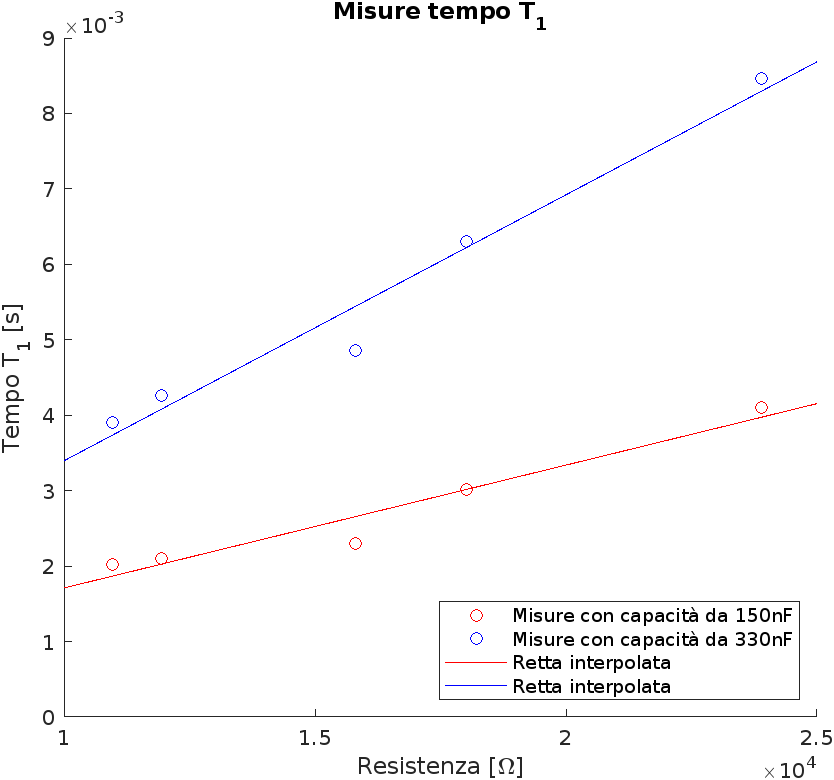
\includegraphics[width=0.5\linewidth]{./ImageFiles/Laboratorio 4/Misure tempo t1}
	\caption{Grafico tempo di carica T\sub{1} in funzione del valore della capacità C e della resistenza R.}
	\label{fig:misure_t1}
\end{figure}
Nelle figure \ref{fig:uscita_circuito_150n} e \ref{fig:uscita_circuito_330n} sono riportate alcune misure dell'intervallo T\sub{1} ottenute tramite i cursori dell'oscilloscopio. Confrontando i valori di T\sub{1} ottenibili dalla equazione \ref{eq:t1} con quelli misurati si può vedere una buona corrispondenza. Per esempio, considerando un valore di R pari a \SI{18.02}{\kilo\ohm} e un valore di capacità \SI{150}{\nano\farad} il valore atteso è di \SI{2.97}{\milli\second}, mentre il valore misurato è di \SI{3.02}{\milli\second}. 

\begin{figure}[h]
	\centering
	\begin{minipage}{.496\textwidth}
		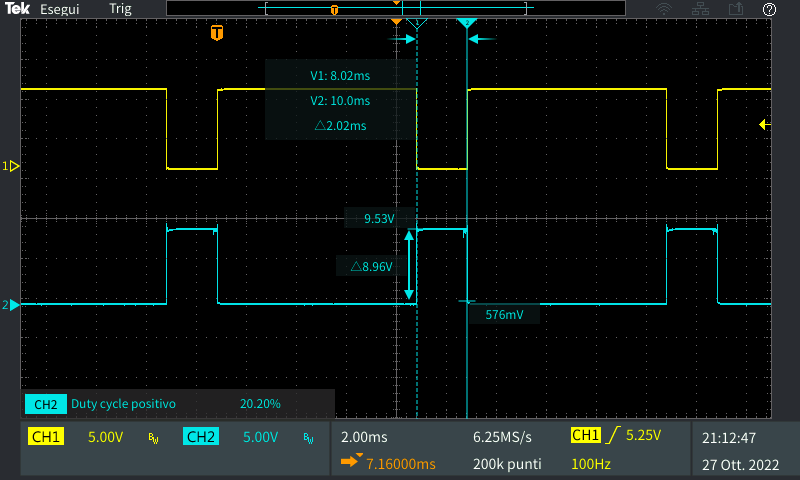
\includegraphics[width=\linewidth]{./ImageFiles/Laboratorio 4/TEK00017.PNG}
	\end{minipage}
	\begin{minipage}{.496\textwidth}
		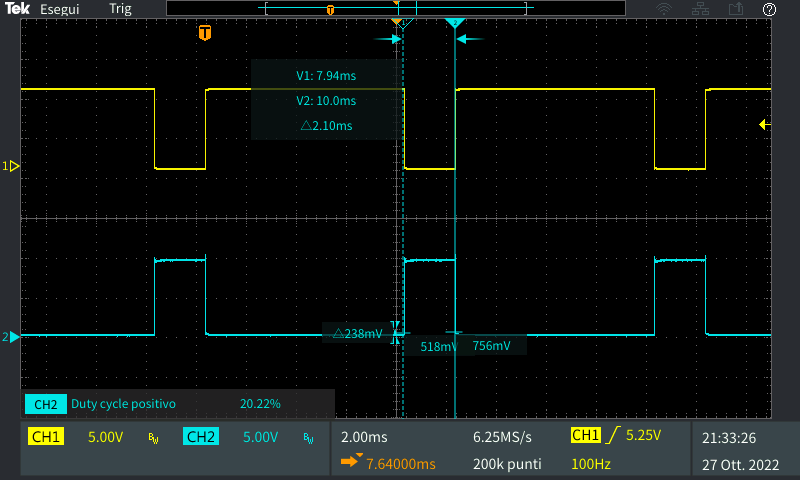
\includegraphics[width=\linewidth]{./ImageFiles/Laboratorio 4/TEK00021.PNG}
	\end{minipage}
	\begin{minipage}{.496\textwidth}
		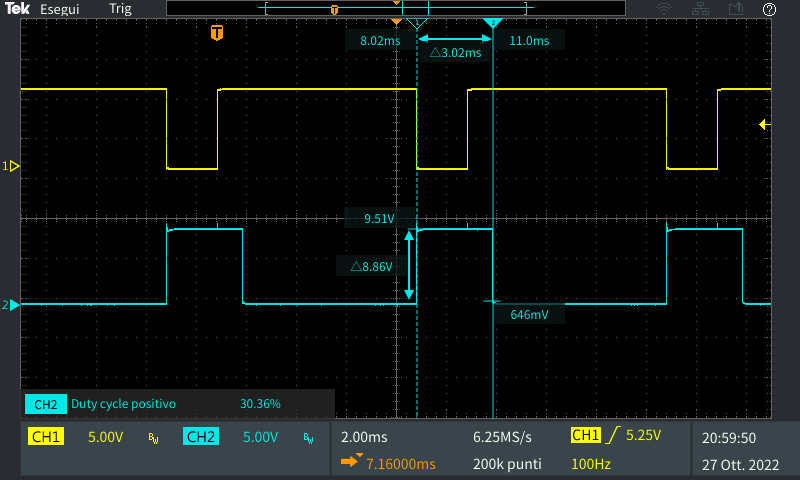
\includegraphics[width=\linewidth]{./ImageFiles/Laboratorio 4/TEK00012.PNG}
	\end{minipage}
	\begin{minipage}{.496\textwidth}
		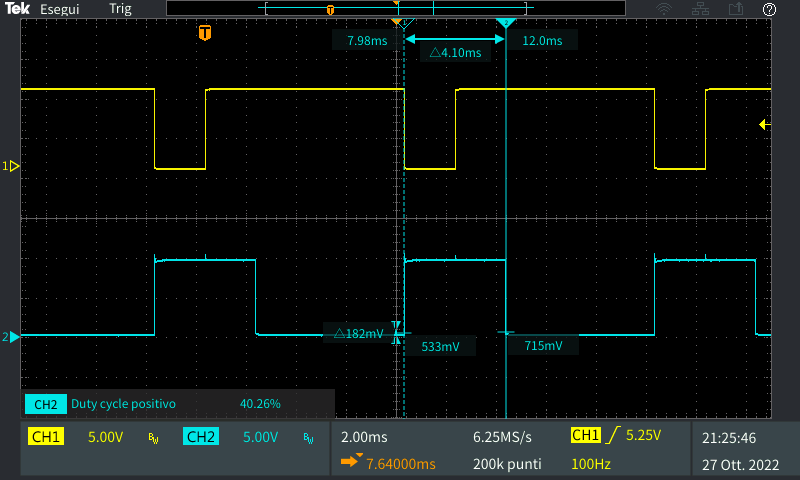
\includegraphics[width=\linewidth]{./ImageFiles/Laboratorio 4/TEK00020.PNG}
	\end{minipage}
	\caption{Misure del segnale in ingresso (linea gialla) e del segnale in uscita (linea azzurra) al circuito. Il segnale in ingresso è una onda quadra di \SI{10}{\volt} picco-picco, con un offset di \SI{5}{\volt}, capacità fissa a \SI{150}{\nano\farad} e resistenza pari a \SI{10,96}{\kilo\ohm} (in alto a sinistra), \SI{11,96}{\kilo\ohm} (in alto a destra), \SI{18,02}{\kilo\ohm} (in basso a sinistra) e \SI{23,90}{\kilo\ohm} (in basso a destra).}
	\label{fig:uscita_circuito_150n}
\end{figure}

\begin{figure}[h]
	\centering
	\begin{minipage}{.496\textwidth}
		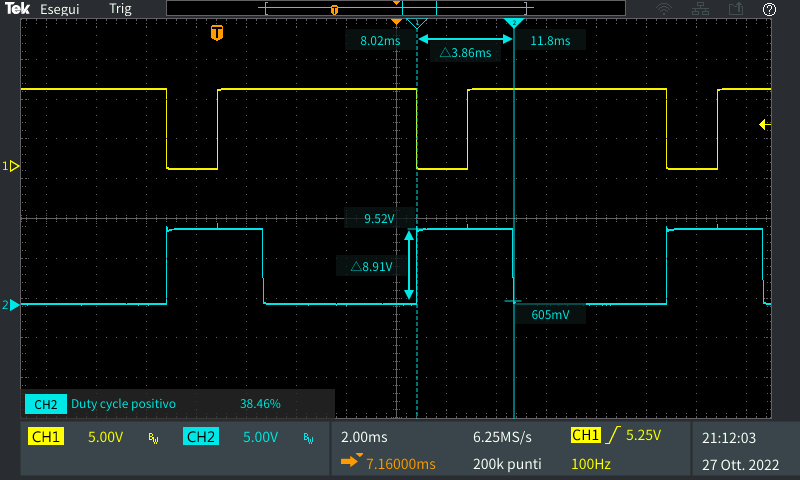
\includegraphics[width=\linewidth]{./ImageFiles/Laboratorio 4/TEK00015.PNG}
	\end{minipage}
	\begin{minipage}{.496\textwidth}
		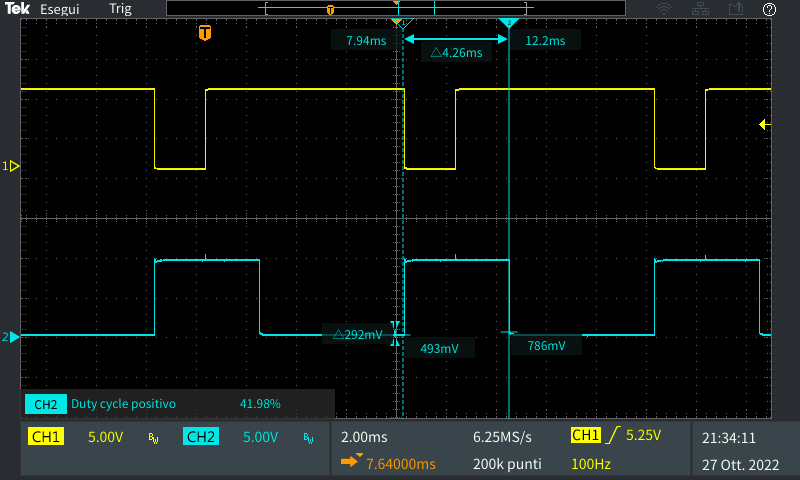
\includegraphics[width=\linewidth]{./ImageFiles/Laboratorio 4/TEK00022.PNG}
	\end{minipage}
	\begin{minipage}{.496\textwidth}
		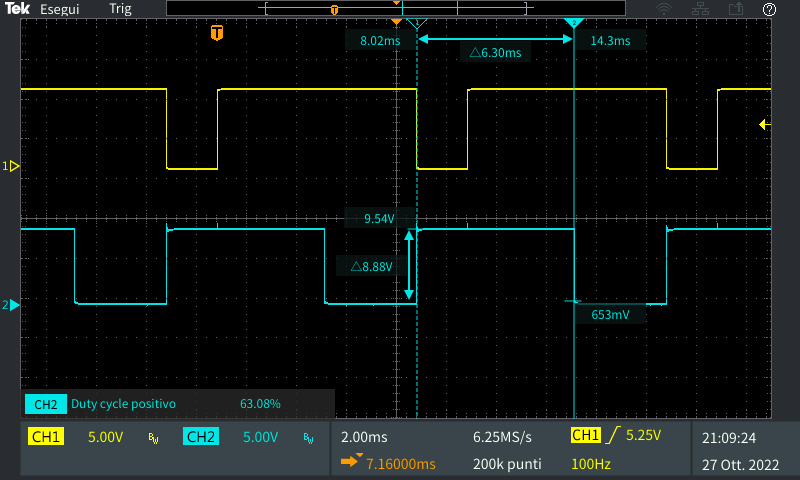
\includegraphics[width=\linewidth]{./ImageFiles/Laboratorio 4/TEK00014.PNG}
	\end{minipage}
	\begin{minipage}{.496\textwidth}
		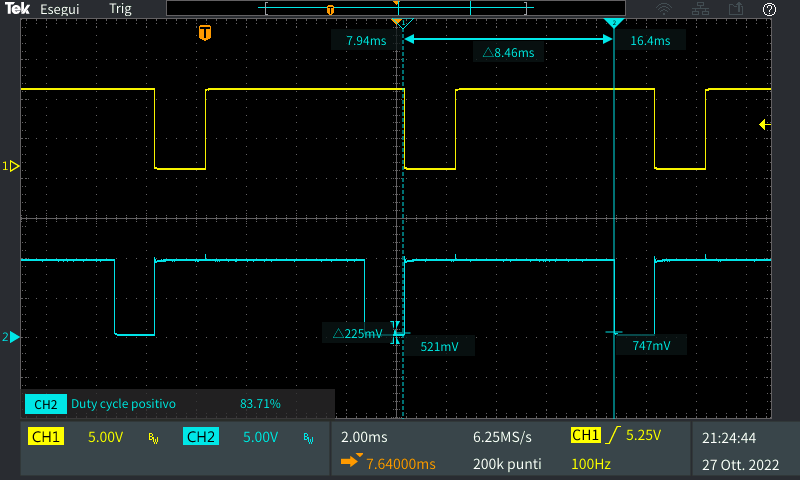
\includegraphics[width=\linewidth]{./ImageFiles/Laboratorio 4/TEK00019.PNG}
	\end{minipage}
	\caption{Misure del segnale in ingresso (linea gialla) e del segnale in uscita (linea azzurra) al circuito. Il segnale in ingresso è una onda quadra di \SI{10}{\volt} picco-picco, con un offset di \SI{5}{\volt}, capacità fissa a \SI{330}{\nano\farad} e resistenza pari a \SI{10,96}{\kilo\ohm} (in alto a sinistra), \SI{11,96}{\kilo\ohm} (in alto a destra), \SI{18,02}{\kilo\ohm} (in basso a sinistra) e \SI{23,90}{\kilo\ohm} (in basso a destra).}
	\label{fig:uscita_circuito_330n}
\end{figure}
